\documentclass{cmc}

\begin{document}

\pagestyle{fancy}
\lhead{\textit{\textbf{Computational Motor Control, Spring 2025} \\
    Python exercise, Lab 3, NOT GRADED}} \rhead{Student \\ Names}

\section*{Student names: \ldots (please update)}

\textit{Instructions: Update this file (or recreate a similar one, e.g.\ in
  Word) to prepare your answers to the questions. Feel free to add text,
  equations and figures as needed. Hand-written notes, e.g.\ for the development
  of equations, can also be included e.g.\ as pictures (from your cell phone or
  from a scanner).  \textbf{This lab is not graded. However, the lab exercises
    are meant as a way to familiarise with dynamical systems and to study them
    using Python to prepare you for the final project.} This file does not need
  to be submitted and is provided for your own benefit. The graded exercises
  will have a similar format.}

\textit{The file \fileref{lab\#.py} is provided to run all exercises in Python.
  % Each \fileref{exercise\#.py} can be run to run an exercise
  % individually.
  % The list of exercises and their dependencies are shown in
  % Figure~\ref{fig:files}.
  When a file is run, message logs will be printed to indicate information such
  as what is currently being run and and what is left to be implemented. All
  warning messages are only present to guide you in the implementation, and can
  be deleted whenever the corresponding code has been implemented correctly.}

% \begin{figure}[ht]
%   \centering 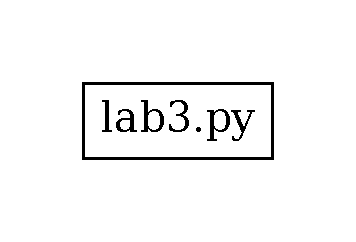
\includegraphics[width=0.5\textwidth]{figures/files}
%   \caption{\label{fig:files} Exercise files dependencies. In this lab, you
%   will be modifying \fileref{exercise3.py}, \fileref{ex3\_pendulum.py},
%   \fileref{exercise4.py} and \fileref{ex4\_hopf.py}.}
% \end{figure}

\section*{Coupled leaky integrator neurons}

\textit{The lab of today is based on a network of two coupled leaky-integrator
  neurons with self- connections as seen in the lecture, and as analyzed in the
  paper:
  \href{https://journals.sagepub.com/doi/10.1177/105971239500300405}{Beer,
    R.D. (1995). On the dynamics of small continuous-time recurrent neural
    networks. Adaptive Behavior 3(4):469-509.} By looking at the Figures 4a-4d
  of that paper, you should be able to reproduce several interesting dynamical
  regimes and answer the questions below. See the file \fileref{lab3.py}}


\subsection*{5.a Set the parameters of the network such as to create a dynamical
  system with \textit{three} fixed points: two stable fixed points and one
  saddle node (check Beer 1995 for ideas and parameter values). Show figures
  that illustrate that behavior. Show or demonstrate the stability of the fixed
  points.}


\begin{figure}[H]
  \centering
  \begin{subfigure}[b]{0.49\textwidth}
    { \centering 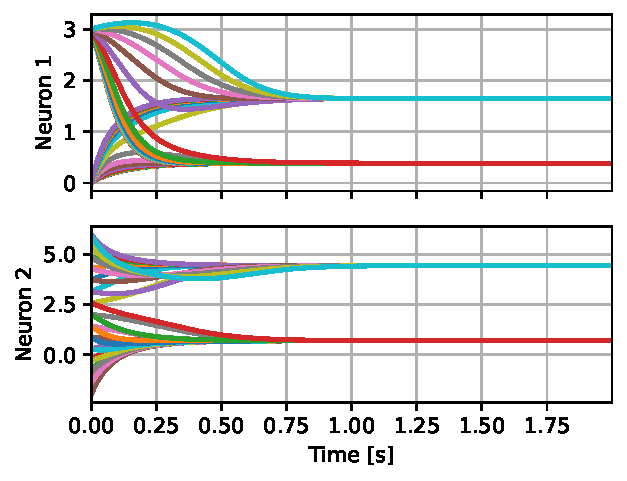
\includegraphics[width=\textwidth]{figures/Case1_state}
      \label{fig:pendulum-basic-state}
    }
    \caption{\corr{Time evolution}}
  \end{subfigure}
  \begin{subfigure}[b]{0.49\textwidth}
    { \centering 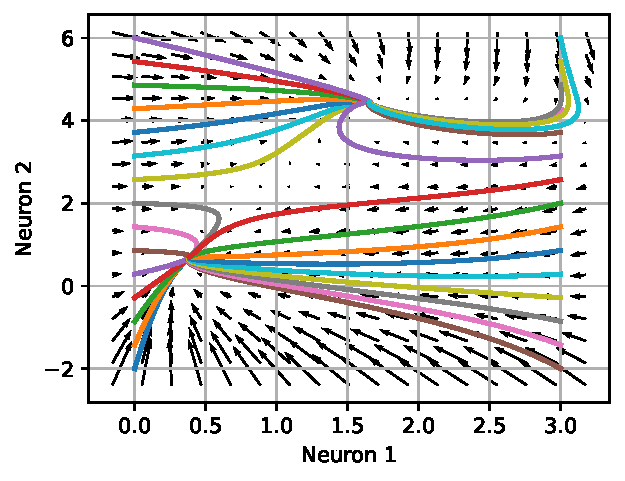
\includegraphics[width=\textwidth]{figures/Case1_phase}
      \label{fig:pendulum-basic-phase}
    }
    \caption{\corr{Phase portrait}}
  \end{subfigure}
  \caption{\corr{This Figure corresponds to the regime shown in figure 4a,
      bottom left in (Beer 1995) (\texttt{b = [-3.4, -2.5]}, \texttt{w = [[5.25,
        1], [-1, 5.25]]}). There are two stable fixed points, and one saddle
      node. The trajectories around the [1, 2.5] area approach towards the
      saddle node, and then convergence to the two different stable fixed
      points. All trajectories converge to one of these stable fixed points.}}
  \label{fig:two-stabe-one-fix}
\end{figure}


\subsection*{5.b Set the parameters of the network such as to create a dynamical
  system with a limit cycle behavior and a single unstable fixed point. Show
  figures that illustrate that behavior. Look also at the behavior of the
  crossing of a Poincaré map (a line in this case). Discuss similarities and
  differences of this neural oscillator with the Hopf oscillator.}


\begin{figure}[H]
  \centering
  \begin{subfigure}[b]{0.49\textwidth}
    { \centering 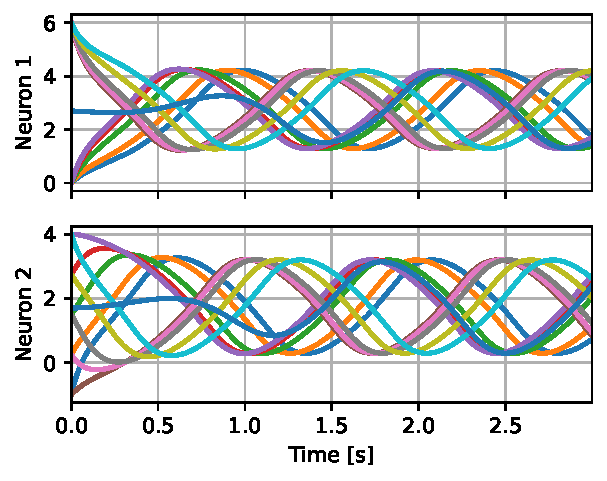
\includegraphics[width=\textwidth]{figures/Case2_state} }
    \caption{\corr{Time evolution}}
  \end{subfigure}
  \begin{subfigure}[b]{0.49\textwidth}
    { \centering 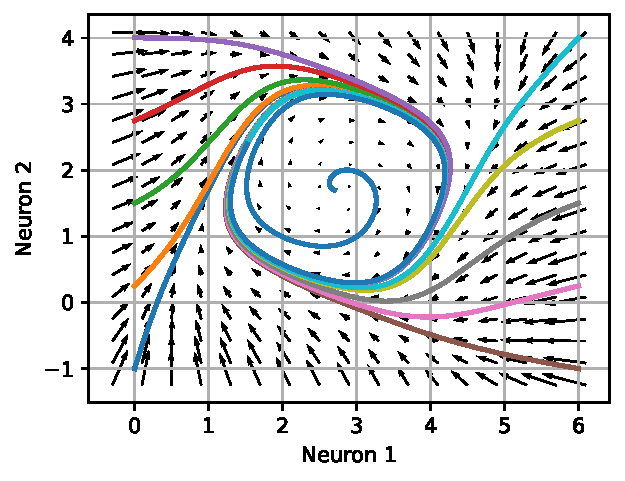
\includegraphics[width=\textwidth]{figures/Case2_phase} }
    \caption{\corr{Phase portrait}}
  \end{subfigure}
  \caption{\corr{This Figure corresponds to the regime shown in figure 4a,
      middle left in (Beer 1995) (\texttt{b = [-2.75, -1.75]}, \texttt{w =
        [[4.5, 1], [-1, 4.5]]}). There is a stable limit cycle, with an unstable
      fixed point inside (as in any limit cycle). From different initial
      conditions, we see convergence to the stable limit cycle.}}
  \label{fig:limit-cycle}
\end{figure}

\corr{We can look at a Poincaré map to see the convergence to the limit cycle:}

\begin{figure}[H]
  \centering
  \begin{subfigure}[b]{0.49\textwidth}
    { \centering 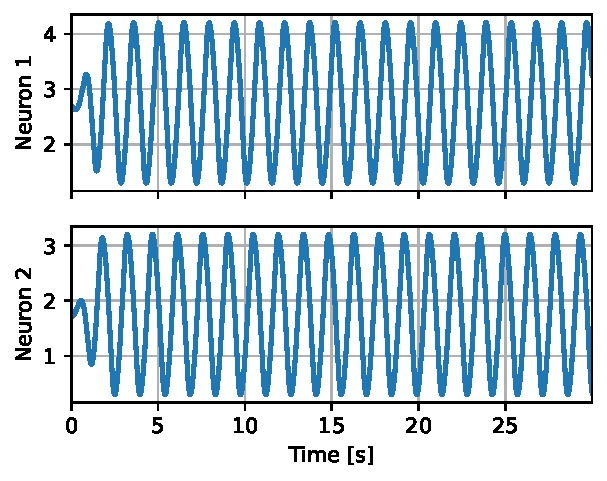
\includegraphics[width=\textwidth]{figures/Case2_cross_state} }
    \caption{\corr{Time evolution}}
  \end{subfigure}
  \begin{subfigure}[b]{0.49\textwidth}
    { \centering 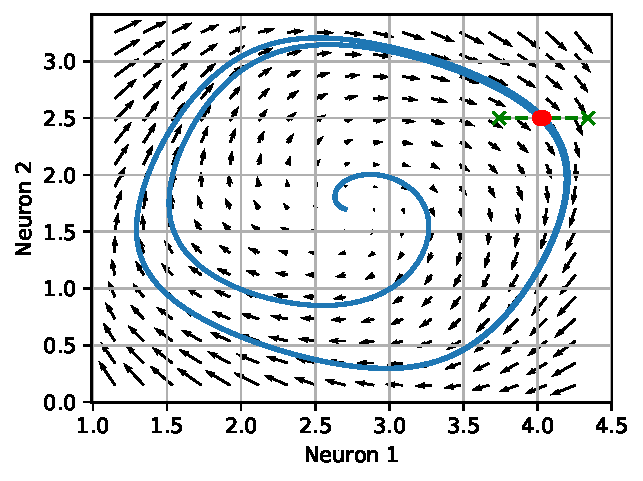
\includegraphics[width=\textwidth]{figures/Case2_cross_phase} }
    \caption{\corr{Phase portrait}}
  \end{subfigure}
  \caption{\corr{System run with initial point \texttt{[2.7, 1.7]}}}
  \label{fig:limit-cycle-poincare}
\end{figure}

\begin{figure}[H]
  \centering
  \begin{subfigure}[b]{0.49\textwidth}
    { \centering
      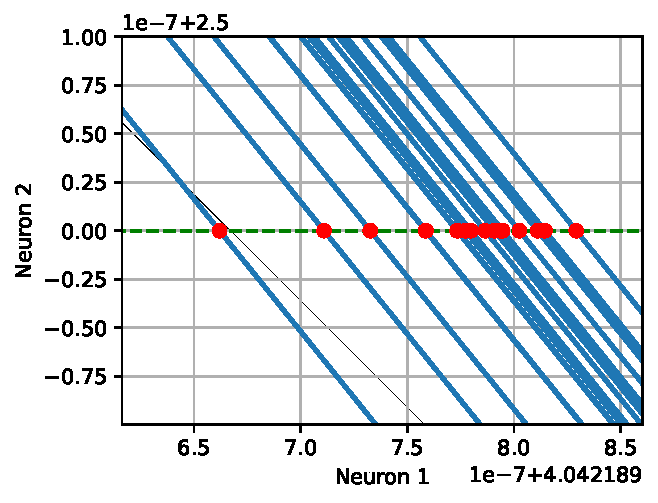
\includegraphics[width=\textwidth]{figures/Case2_cross_phase_zoom} }
    \caption{\corr{Crossings of the Poincaré section}}
  \end{subfigure}
  \begin{subfigure}[b]{0.49\textwidth}
    { \centering 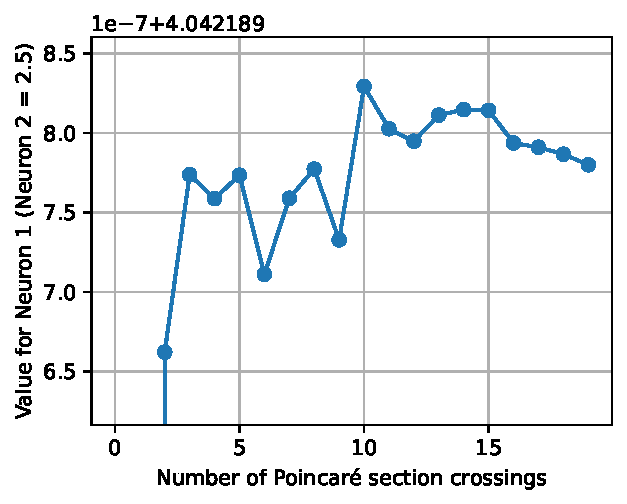
\includegraphics[width=\textwidth]{figures/Case2_cross} }
    \caption{\corr{Poincaré map}}
  \end{subfigure}
  \caption{\corr{Crossings of the Poincaré section (left) lead to a Poincaré map
      (right) in which the states rapidly converge to an almost constant
      value and oscillates around it. The numerical integration leads to
      these negligible numerical artefacts (error $\sim 10^{-7}$). To have a
      better way to detect crossings we can use interpolation and/or
      finer integration steps. However, at steady state, a similar error would appear. }}
  \label{fig:limit-cycle-poincare-analysis}
\end{figure}

\corr{\textbf{Similarities with Hopf:}} \corr{
  \begin{itemize}
  \item Stable limit cycle behavior
  \item Basin of attraction = whole state space (except unstable fixed point
    within the limit cycle)
  \item Two dimensional oscillators
  \end{itemize}
}

\corr{\textbf{Differences:}} \corr{
  \begin{itemize}
  \item The shape of the limit cycle is different (harmonic, i.e.\ sin and cos,
    circle shape for Hopf, more complex shape here)
  \item Vector field is not symmetric, convergence strength varies dependent on
    angle
  \item Angle is not the phase
  \item Not as simple to make a bifurcation between between single point
    attractor and limit cycle (but must be possible)
  \end{itemize}
}


\subsection*{5.c Set the parameters of the network such as to create a dynamical
  system with a limit cycle behavior and three fixed points: a single unstable
  fixed point, a single saddle node, and a single stable fixed point. Show
  figures that illustrate that behavior. Discuss similarities and differences
  with the Hopf oscillator. Discuss whether such a system could have interesting
  properties for motor control.}


\begin{figure}[H]
  \centering
  \begin{subfigure}[b]{0.49\textwidth}
    { \centering 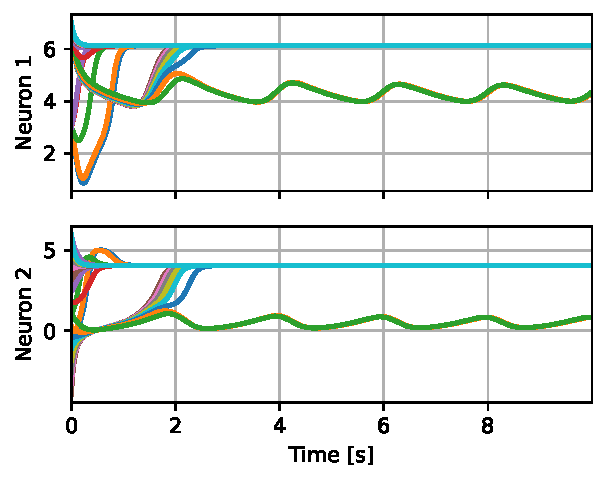
\includegraphics[width=\textwidth]{figures/Case3_state} }
    \caption{\corr{Time evolution}}
  \end{subfigure}
  \begin{subfigure}[b]{0.49\textwidth}
    { \centering 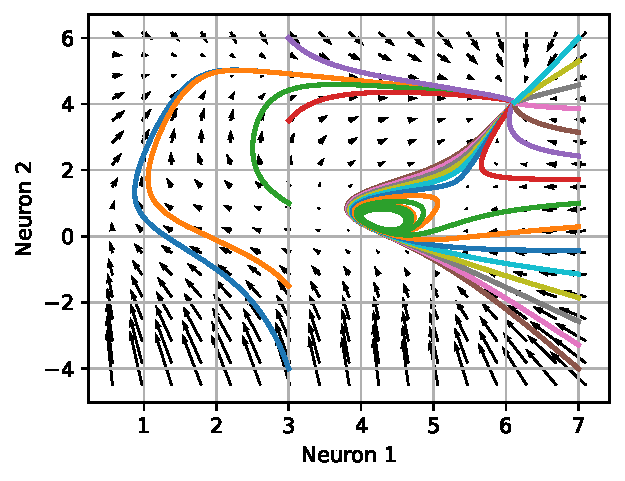
\includegraphics[width=\textwidth]{figures/Case3_phase} }
    \caption{\corr{Phase portrait}}
  \end{subfigure}
  \caption{\corr{This Figure corresponds to the regime shown in figure 4b,
      middle left in (Beer 1995) (\texttt{b = [-3.233, -1.75]}, \texttt{w =
        [[5.5, 1], [-1, 5.5]]}).}}
  \label{fig:stable-unstable-cycle}
\end{figure}

\corr{\textbf{Similarities and differences:}}

\corr{Like 5b.\ but additional difference: basin of attraction to limit cycle is
  not the whole space anymore, only a subpart, because of the added stable fixed
  point which has its own, larger, basin of attraction.}

\begin{figure}[H]
  \centering
  \begin{subfigure}[b]{0.49\textwidth}
    { \centering 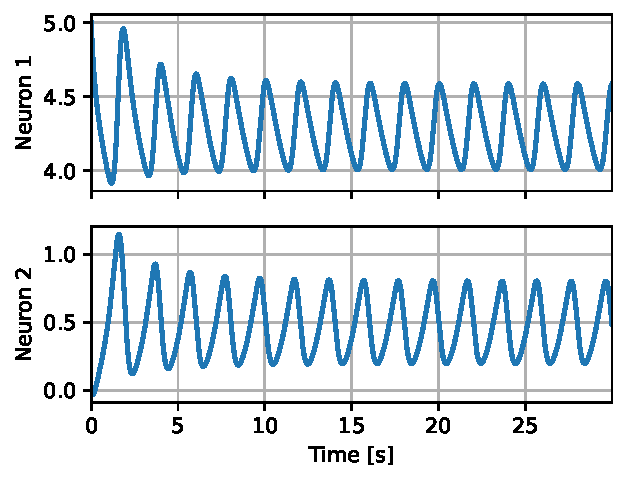
\includegraphics[width=\textwidth]{figures/Case3_cross_state} }
    \caption{\corr{Time evolution}}
  \end{subfigure}
  \begin{subfigure}[b]{0.49\textwidth}
    { \centering 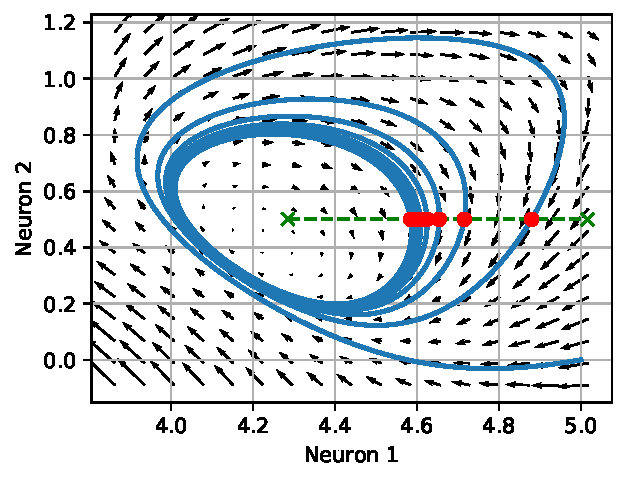
\includegraphics[width=\textwidth]{figures/Case3_cross_phase} }
    \caption{\corr{Phase portrait}}
  \end{subfigure}
  \caption{\corr{System run with initial point \texttt{[5, 0.0]}}}
  \label{fig:stable-unstable-cycle-poincare}
\end{figure}

\begin{figure}[H]
  \centering
  \begin{subfigure}[b]{0.49\textwidth}
    { \centering
      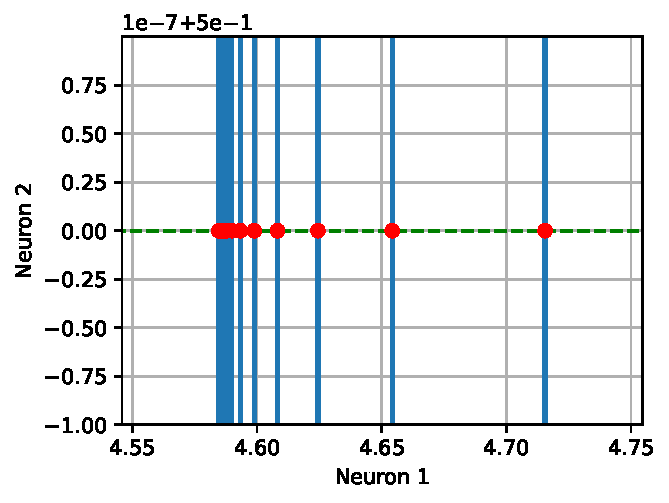
\includegraphics[width=\textwidth]{figures/Case3_cross_phase_zoom} }
    \caption{\corr{Crossings of the Poincaré section}}
  \end{subfigure}
  \begin{subfigure}[b]{0.49\textwidth}
    { \centering 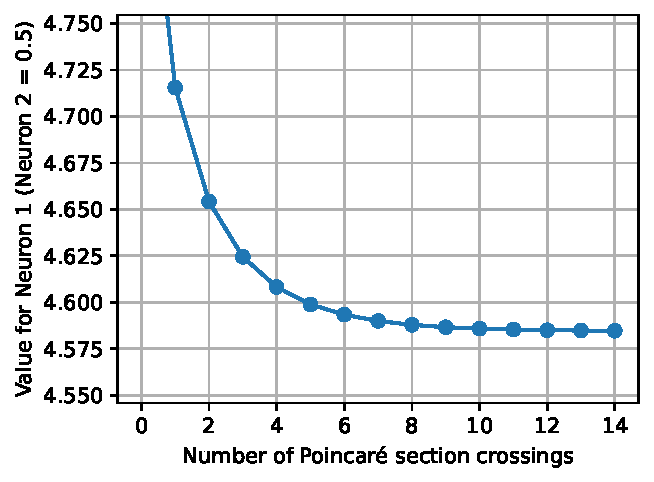
\includegraphics[width=\textwidth]{figures/Case3_cross} }
    \caption{\corr{Poincaré map}}
  \end{subfigure}
  \caption{\corr{Poincaré analysis}}
  \label{fig:stable-unstable-cycle-poincare-analysis}
\end{figure}




\end{document}